We refer to the specific value of the factorization scale at which the number
of active flavors is changing from $n_f$ to $n_f+1$ (or vice-versa) as the
threshold $\mu_h$. Although this value usually coincides with the respective
quark mass $m_h$, \eko{} implements the explicit expressions when the two
scales do not match. This variation can be used to estimate \mhou{}~\cite{AbdulKhalek:2019ihb}.

\begin{figure}
    \centering
    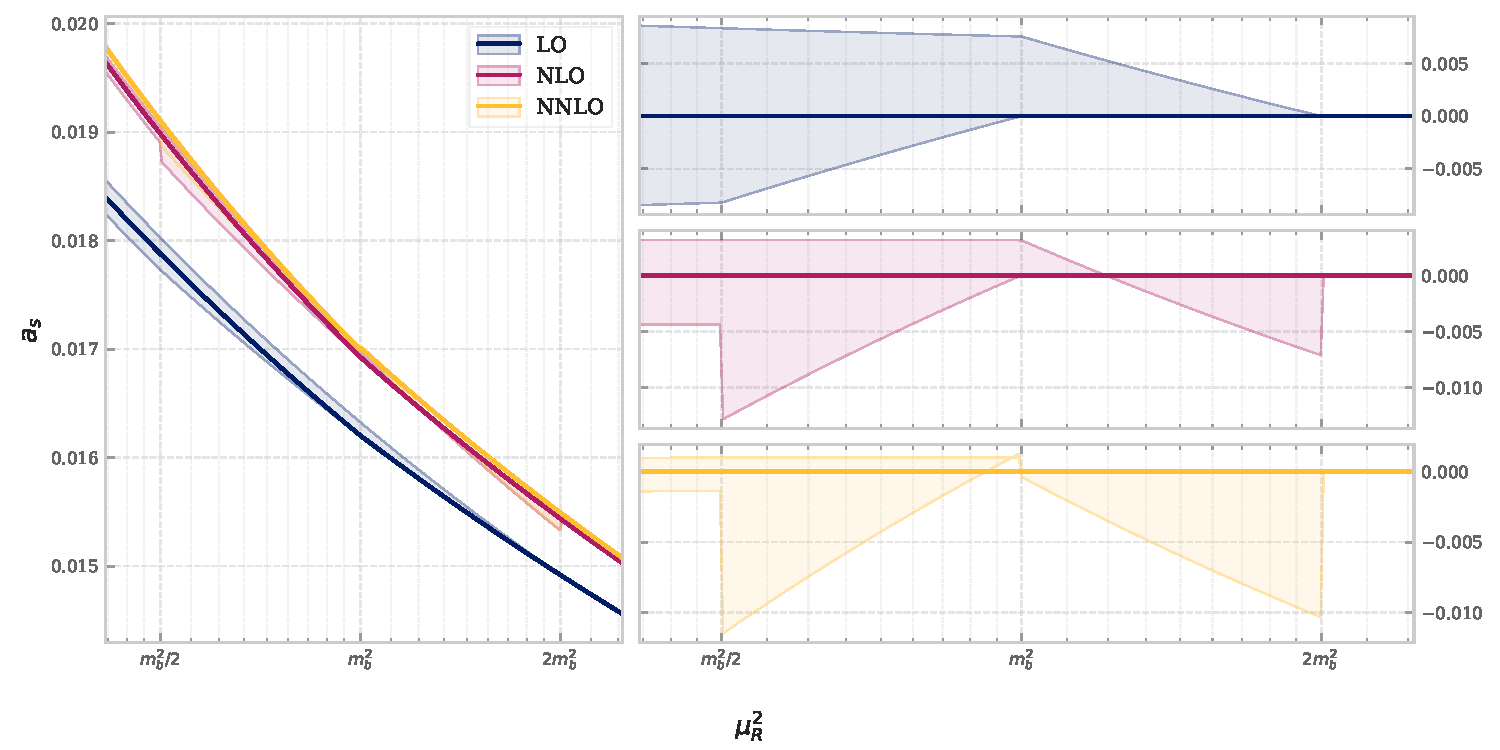
\includegraphics[width=\textwidth]{ch-eko/strong_coupling}
    \caption{Strong coupling evolution $a_s(\mu_R^2)$ at \lo{},
    \nlo{} and \nnlo{}
    respectively with the bottom matching $\mu_b^2$ at $1/2, 1,$ and $2$ times the
    bottom mass $m_b^2$ indicated by the band. In the left panel we show the absolute
    value, while on the right we show the ratio towards the central scale choice.
     \label{fig:asmatching}}
\end{figure}

In \cref{fig:asmatching} we show the strong coupling evolution $a_s(\mu_R^2)$
around the bottom mass with the bottom threshold $\mu_b^2$ eventually not coinciding
with the respective bottom quark mass $m_b^2$.
The dependency on the \lo{} evolution is only due to the change of active
flavor in the beta function ($\beta_0 = \beta_0(n_f)$), which can be seen in
the ratio plot by the continuous connections of the lines.
At \nlo{} evolution the matching condition already becomes discontinuous for
$\mu_h^2 \neq m_h^2$, represented in the ratio plot by the offset for the
matched evolution. 
The matching for the \nnlo{} evolution~\cite{Chetyrkin:2005ia,Schroder:2005hy}
is intrinsically discontinuous, which is indicated in the ratio plot by the
discrete jump at the central scale $\mu_R^2 = m_b^2$.
For $\mu_R^2 > 2m_b^2$ the evolution is only determined by the reference value
$a_s(m_Z^2)$ and the perturbative evolution order.
For $\mu_R^2 < m_b^2/2$ we can observe the perturbative convergence as the
relative difference shrinks with increasing orders.
Since it is converging, the effect of the matching condition should cancel more
and more exactly with the difference in running, but the magnitude of both is
increasing with the order, since the perturbative expansion of the beta
function $\beta(a_s)$ is a same sign series.

\begin{figure}
    \centering
    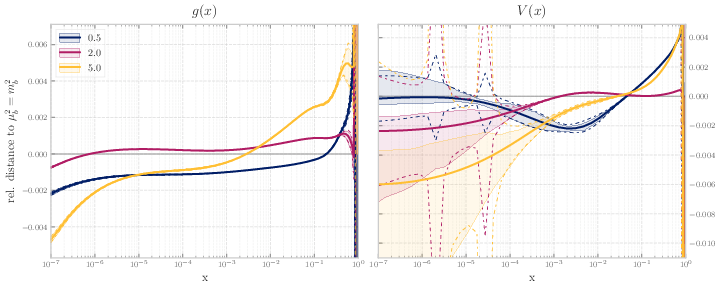
\includegraphics[width=\textwidth]{ch-eko/matching-b-thr}
    \caption{Difference of \pdf{} evolution with the bottom matching $\mu_b^2$ at $1/2, 2,$ and
        $5$ times the bottom mass $m_b^2$ relative to $\mu_b^2 = m_b^2$. Note
        the different scale for the two distributions.  All evolved in
        $\muF^2=\SI[parse-numbers=false]{1.65^2\to 10^4}{\GeV^2}$.}
    \label{fig:pdfmatching}
\end{figure}

In \cref{fig:pdfmatching} we show the relative difference for the \pdf{} evolution with
threshold values $\mu_h^2$ that do not coincide with the respective heavy
quark masses $m_h^2$. When matching at a lower scale the difference is
significantly more pronounced as the evolution includes
a region where the strong coupling varies faster. When dealing 
with $\mu_h^2 \neq m_h^2$ the \pdf{} matching conditions become discontinuous
already at \nlo{}~\cite{Buza_1998}. These contributions are also available in
\apfel{}~\cite{Bertone:2013vaa}, but not in \pegasus{}~\cite{Vogt:2004ns} and although they are present in the code
of \qcdnum{}~\cite{Botje:2010ay} they can not be accessed there.
For the study in \cite{Ball:2022qks} we also implemented the \pdf{} matching at
\nnnlo{}~\cite{Bierenbaum:2009zt,Bierenbaum:2009mv,Ablinger:2010ty,Ablinger:2014vwa,Ablinger:2014uka,Behring:2014eya,Ablinger_2014,Ablinger_2015,Blumlein:2017wxd}.
